\documentclass{article}

\usepackage{geometry}
\usepackage{makecell}
\usepackage{array}
\usepackage{multicol}
\usepackage{setspace}
\usepackage{hyperref}
\usepackage{changepage}
\usepackage{booktabs}
\usepackage{cprotect}
\usepackage{tabularx}
\usepackage{graphicx}
\usepackage{fancyvrb}
\usepackage[explicit]{titlesec}
\usepackage{float}
\newcolumntype{?}{!{\vrule width 1pt}}
\DefineShortVerb{\Ħ}
\newcommand{\paragraphlb}[1]{\paragraph{#1}\mbox{}\\}
\renewcommand\theadalign{tl}
\setstretch{1.10}
\setlength{\parindent}{0pt}

\titleformat{\section}
  {\normalfont\Large\bfseries}{\thesection}{1em}{\hyperlink{sec-\thesection}{#1}
\addtocontents{toc}{\protect\hypertarget{sec-\thesection}{}}}
\titleformat{name=\section,numberless}
  {\normalfont\Large\bfseries}{}{0pt}{#1}

\titleformat{\subsection}
  {\normalfont\large\bfseries}{\thesubsection}{1em}{\hyperlink{subsec-\thesubsection}{#1}
\addtocontents{toc}{\protect\hypertarget{subsec-\thesubsection}{}}}
\titleformat{name=\subsection,numberless}
  {\normalfont\large\bfseries}{\thesubsection}{0pt}{#1}

\hypersetup{
    colorlinks,
    citecolor=black,
    filecolor=black,
    linkcolor=black,
    urlcolor=black
}

\geometry{top=12mm, left=1cm, right=2cm}
\title{\vspace{-1cm} Netzwerktechnologien 1}
\author{Andreas Hofer}

\begin{document}
	\maketitle
	\tableofcontents
	\section{Grundlagen}
	Netzwerke sind Verbindungen zwischen Personen aber auch Geräten, welche miteinander kommunizieren können. Netzwerke können eine beträchtliche Größe annehmen, wobei selbst ein Heimnetzwerk einige Teilnehmer ausmachen kann. Aufgabe eines Computernetzwekes ist, Teilnehmer miteinander kommunizieren zu lassen und Ressourcen auszutauschen. Der Name \textit{Internet} stammt auch aus diesem Konzept, nämlich dem \textit{\textbf{Inter-Net}working}. \\
	Für ein Netzwerk benötigt man:
	\begin{itemize}
	 	\item{Zumindest zwei Teilnehmer. Bei nur einem Teilnehmer gibt es ja nichts zu kommunizieren.}
	 	\item{Zusätzlich braucht man ein Medium zur Übertragung wie Kabel oder Antennen.}
	 	\item{Netzwerkprotokolle. Gleich wie man bei menschlicher Kommunikation gewisse Normen hat, muss man sich auch in einem Netzwerk an Konventionen halten.}
	 \end{itemize}
	 Erste Netzwerke wurden bereits in dne 60er Jahren aufgebaut, als in den USA 4 Universitäten den Vorläufer des ARPANETS aufbauten um miteinander kommunizieren zu können. In den 90er Jahren wurden PCs und Netzwerktechnologien weiter verbreitet, was auch zu einer weiteren Akzeptanz führte. \\
	 \subsection{Nachrichtenübertragung}
	 Um Nachrichten zu übertragen gibt es zwei Wege die Kommunikation zu gewährleisten: Circuit- und Packet Switching. \\
	 Bei Circuit Switching gibt es eine direkte Leitung zwischen zwei Teilnehmern, welche direkt miteinander kommunizieren und exklusiv zur Verfügung stehen. Frühe Telefonnetzwerke bauten auf Circuit Switching auf indem Schalteinrichtungen zuerst händisch und später elektronisch eine Leitung zwischen den Parteien aufbaute. \\
	 Die alternative und bedeutend effektivere Methode ist Packet Switching. Alle Teilnehmer sind miteinander verbunden, jedoch werden Dateien die über das Netzwerk gesendet werden in gleich große Pakete aufgeteilt und erst am Zielort wieder zusammengebaut wodurch das Netzwerk nicht durch eine große Datei exklusiv beansprucht wird. Das Internet basiert heutzutage exklusiv auf Packet Switching. \\
	 \subsection{Netzwerktopologien}
	 Netzwerke können in verschiedenen Topologien zusammengeschlossen sein. Diese können entweder logische oder physikalische Topologien sein. Die vier Grundtopologien sind:
	 \begin{itemize}
	 	\item{Bus}
	 	\begin{itemize}
	 		\item{Teilnehmer liegen an einem gemeinsamen Kabel und sind so parallel geschalten. Dadurch fällt das Netzwerk nicht aus, selbst wenn ein Teilnehmer ausfällt.}
	 	\end{itemize}
	 	\item{Ring}
	 	\begin{itemize}
	 		\item{Im Ring sind Teilnehmer in Serie verbunden. Nachteile dieser Topologie sind, dass eine Nachricht stets alle Teilnehmer durchlaufen muss um zum Ziel zu kommen. Ebenfalls fällt das System aus, wenn ein Teilnehmer ausfällt.}
	 	\end{itemize}
	 	\item{Stern}
	 	\begin{itemize}
	 		\item{In einem Stern sind alle Teilnehmer nicht untereinander sondern mit einem Switch oder einem Hub verbunden. So agiert der Switch als Mediator zwischen den Teilnehmern im Netzwerk. Wenn jedoch der Switch/Hub ausfällt, fällt das gesamte Netzwerk aus. Viele Heimnetzwerke sind so aufgebaut.}
	 	\end{itemize}
	 	\item{Maschen}
	 	\begin{itemize}
	 		\item{Jeder Knoten ist mit einer Vielzahl an anderen Teilnehmern verbunden. Theoretisch könnte jeder Teilnehmer mit jedem Teilnehmer verbunden sein, was jedoch wenige Vorteile bietet. Dieses System ist sehr ausfallsicher, da eine Alternativroute gefunden werden kann, falls eine direkte Verbindung ausfällt. Das Internet baut in großen Teilen auf einem Maschennetzwerk auf.}
	 	\end{itemize}
	 \end{itemize}
	 \subsection{Client-Server Modell}
	 Bei einem Client-Server Modell wird von dem Server eine Dienstleistung angeboten, welche von einem Client in Anspruch genommen wird. Clients sind üblicherweise Endbenutzergeräte. Wenn man mit einem Browser eine Website aufruft, ist der Webserver der Server, welcher dem Browser als Client die Website überträgt. \\
	 \subsection{Bandbreite und Latenz}
	 Bandbreite und Latenz sind entscheidende Faktoren für die Effektivität eines Netzwerkes.\\
	 \begin{itemize}
	 	\item{Die Bandbreite sagt aus wie viele Daten in einem Zeitraum über das Netzwerk übertragen werden können. Es wird meistens in MBit oder MByte gemessen.}
	 	\item{Latenz ist die Verzögerung mit welcher das Signal verarbeitet oder übertragen wird. Wenn ein Server beispielweises sehr weit entfernt ist, kann trotz der Lichtgeschwindigkeit des Signals eine merkliche Latenze entstehen.}
	 \end{itemize}
	 \subsection{Reichweiten}
	 Netzwerke können unterschiedliche Ausdehnungen haben, was auch beeinflusst wie viele Nutzer meist in ihnen angemeldet sind:
	 \begin{itemize}
	 	\item{PAN (Personal Area Network) - Sehr geringe Distanz (1m) so wie die Verbindung zwischen einem Köpfhörer und einem Handy.}
	 	\item{LAN (Local Area Network) - Relativ große Distanz (bis zu 5km), kann jedoch auch nur das private Hausnetzwerk sein.}
	 	\item{MAN (Metropolitan Area Network) - Das Netzwerk einer Stadt wie beispielweise ein Fernsehkabel.}
	 	\item{WAN (Wide Area Network) - Ein Netzwerk welches ein gesamtes Land überspannt. Das US-Militär besitzt ein eigenes Netzwerk, welches ein WAN ist.}
	 	\item{GAN (Global Area Network) - Das Internet das den Globus umspannt}
	 \end{itemize}
	 \subsection{Wer verwaltet das Internet?}
	 \subsubsection{ISPs}
	 Es gibt verschiedene ISP Einteilungen, welche nach Größe und Systemrelevanz gestaffelt sind.
	 \begin{itemize}
	 	\item{Tier 1 - Betreiber des globalen Internet-Backbones. Besitzen oft eigene Netzwerke (z.B. Deutsche Telekom)}
	 	\item{Tier 2 - Betreiber eines lokalen Netzwerkes (z.B. A1)}
	 	\item{Tier 3 - Ein kleiner Betreiber, welcher Dienste an den Endkunden verkauft. (z.B. Energie Steiermark)}
	 \end{itemize}
	 Diese verschiedenen Tiers der Betreiber verkaufen Zugang zu ihrem Netzwerk an niedrigere Tiers.
	 \subsubsection{IETF}
	 Jedoch muss es jemanden geben, welcher zum Beispiel IP Addressen oder anderes verwaltet. \\
	 Eine solche Organisation ist die Internet Engineering Taskforce (IETF), welche jedoch keine Weisungsgewalt besitzt. Innerhalb dieser Taskforce bestehen bis zu 100 Working Griups welche gemeinsam Drafts ausarbeiten. Dabei muss nur ein grober Konsens zur Entscheidungsfindung bestehen wobei jeder mitmachen kann. \\
	 Ein erfolgreicher Draft kann zu einem Request for Comments (RFC) werden, welche Diskussionen zu einer Veröffentlichung erbitten. Viele veröffentlichte RFCs gelten heute als Internetstandard (z.B. RFC 791 für IPv4).
	 \subsubsection{IEEE, W3C, IANA}
	 Weitere Organisationen sind das Institute of Electrical and Electronics Engineers, welche Übertragungsstandards verwaltet. \\
	 Das World Wide Web Consortium ist stattdessen für die Webstandards wie HTML und XML verantwortlich. \\
	 Die Internet Assigned Numbers Authority (IANA) verwaltet IP- sowie Web Adressen. 
	 \section{Schichtenmodell}
	 Das OSI Schichten Modell verwaltet den Ablauf einer Internetübertragung indem jedes Packet die einzelnen Schichten durchlaufen muss. Diese Schichten bauen stets aufeinander auf und haben eine spezifische Ausgabe. Also ist jede der Schichten abhängig davon, dass die anderen Schichten ihre Arbeit vollrichten. Jede Schicht kommuniziert nur mit der gleichen Schicht beim Empfänger und fügt hiefür zusätzliche Information hinzu, welche von der anderen Schicht verwendet wird. Einige Schichtenmodelle sind:
	 \begin{itemize}
	 	\item{Das OSI Schichten Modell}
	 	\item{Das TCP/IP Modell}
	 	\item{Das Hybride Referenzmodell}
	 \end{itemize}
	 Das OSI Modell ist der Standard welcher normalerweise das Internet bzw. das Netzwerk beschreibt. Es wurde 1983 von der ISO veröffentlicht. Das TCP/IP Modell wurde in den 70er Jahren entwickelt und war bereits der Standard als das OSI Modell implementiert wurde. Das Problem war, dass ein Großteil des Internets bereits auf dem TCP/IP aufgebaut war und Anbieter hatten wenig Interesse daran, dies zu ändern. \\
	 Die Konsequenz davon ist, dass heutzutage immer noch das TCP/IP Modell Anwendung findet jedoch in gewissen Teilen von dem OSI Modell beinflusst wurde. Zur Vereinfachung wird ein Hybrides Referenzmodell beschrieben, welches die zwei Modelle teilweise kombiniert. Das Modell besteht aus:
	 \begin{itemize}
	 	\item{Anwendungsschicht - Relevante Daten (z.B. eine Email)}
	 	\item{Transportschicht - Die Daten werden in Segmente geteilt (z.B. mittels TCP)}
	 	\item{Vermittlungsschicht - Die logische Adresse wird hinzugefügt und in Pakete verpackt (z.B. mittels IP)}
	 	\item{Sicherungsschicht - Die Physische Adresse wird hinzugefügt (z.B. die MAC Adresse)}
	 	\item{Bitübertragungsschicht - Die Teile werden in physische Bits verwandelt, damit sie übertragen werden können.}
	 \end{itemize}
	 Diese Schichten bauen auf Protokollen auf, welche von beiden verstanden werden, womit diese Informationen austauschen können. Ein Beispiel eines Protokolls ist eine Begrüßungsfloskel zwischen Bekannten. Konkretes Netzwerkbeispiel ist der TCP Handshake, in welchem die beiden Teilnehmer dreifach sicherstellen, dass sie erfolgreich kommunizieren. \\
	 Jede Schicht hat genaue Verantwortungen, während die genauen Details von Provider zu Provider jedoch unterschiedlich sind. Da jede Schicht ein abgeschlossenes System ist, kann man die Vorgänge einer Schicht ersetzen und muss das restliche System nicht verändern. \\
	 Wenn die Information die Schichten durchläuft, wird diese jeweils mit Zusatzinformation versehen. Diesen Prozess nennt man Verkapselung, da eine Kapsel um die Information sowie die anderen Kapseln gelegt wird. Diese Kapsel wird jeweils von der gleichen Schicht beim Empfänger wieder entpackt unt verwertet. Der Prozess funktioniert beispielsweise:
	 \begin{enumerate}
	 	\item{Daten werden von der Anwendungsschicht erzeugt.}
	 	\item{Die Transportschicht fügt einen Header hinzu.}
	 	\item{Die Vermittlungsschicht fügt einen weiteren Header hinzu.}
	 	\item{Die Sicherungsschicht fügt jeweils einen Header und einen Trailer hinzu.}
	 	\item{Die Übertragungsschicht überträgt die Daten und gibt an, wann die Übertragung beginnt und endet.}
	 \end{enumerate}
	 Aus diesem Grund kann man sich die Schichten wie eine Matryoshka-Puppe vorstellen, wo mehr Puppen um die Puppe gestapelt werden. \\
	 Die verschiedenen Schichten stellen sicher, dass jeweils keine Probleme bei der Übertragung entstehen.
	 \begin{itemize}
	 	\item{In der Bitübertragungsschicht wird die Integrität der physischen Verbindung sichergestellt.}
	 	\item{Die Sicherungsschicht stellt sicher, dass das Übertragungsmedium fehlerfrei agiert.}
	 	\item{Die Vermittlungsschicht vermittelt Pakete zwischen logischen Netzen innerhalb eines Netzwerkes.}
	 	\item{Die Transportschicht stellt sicher, dass die Daten zwischen den Prozessen auf unterschiedlichen Geräten übertragen werden.}
	 \end{itemize}
	 \section{Bitübertragungsschicht}
	 Die Bitübertragungsschicht befasst sich mit der Frage, wie kommen die Bits physisch von einem Gerät zum anderen? Dieser physische Anschluss muss nicht in Form eines Kabels sein, sondern kann auch ein WLAN Sender oder Empfänger sein. \\
	 Hierbei kodiert der Sender die Dateien mit Leitungscodes in Signale und der Empfänger dekodiert diese Signale erneut.
	 \subsection{Kabelgebundene Medien}
	 Das Übertragungsmedium bestimmt hierbei mit welcher Geschwindigkeit die Daten übertragen werden können. Kabelgebundene Medien können Twisted-Pair Kabel oder Koaxialkabel sein, aber auch Glasfaserkabel. \\
	 Twisted-Pair Kabel haben paarweise zusammengedrehte Kabel um die Interferenz auszugleichen. Diese Kabel haben unterschiedliche Leistungskategorien wobei Cat-5 Kabeln bis zu 1 Gbit an Daten übertragen kann. Glasfaserkabel hingegen arbeiten mit Lichtleitern, wodurch viel höhere Übertragungsraten erreicht werden können. \\
	 \subsection{Kabellose Medien}
	 Bei kabellosen Medien werden diese stattdessen mittels Energiewellen übertragen. Die bekannteste kabellose Technologie ist das WLAN, welches für eher kleinere Bereiche konzipiert worden ist. WLAN verwendet spezifische Frequenzbereiche, wobei WLAN zwischen 2,4 - 2,48 GHz und 5,15 - 5,725 GHz. Diese Blöcke werden jeweils in Kanäle unterteilt, wobei der 2,4GHz Bereich in 13 Blöcke unterteilt ist. Standards in der kabellosen Technologie können sich drastisch in ihrer Übertragungsrate unterscheiden. \\
	 \subsubsection{Kommunikation zwischen Geräten}
	 Geräte können auf verschiedenen Wegen miteinander verbunden sein. Eine Verbindungsart ist der Ad-Hoc Modus, in welchem Endgeräte ein vermaschtes Netz bilden und jedes Gerät mit jedem anderen Gerät verbunden sein kann. Alternativ dazu und weiter verbreitet ist der Infrakstrukturmodus. Hier gibt es eine Basisstation, wie ein Access Point oder Router, welche sich periodisch mit allen Endgeräten verbindet und den Netzwerknamen und die Liste der unterstützten Übertragungsraten verwaltet.
	 \subsubsection{Herausforderungen kabelgebundener Medien}
	 Eine der Herausforderungen der Verbindung zwischen Geräten ist das Fading, wobei die Signalstärke sehr von Hindernissen wie Wände beeinflusst werden kann. Die Mehrwegausbreitung kann auch dazu führen, dass Signale reflektiert werden und dadurch ungeordnet am Empfänger ankommt. Interferenz aus anderen Quellen kann auch zu einer Beeinträchtigung der Signalstärke führen. Elektromagnetisches Rauschen kann schwächere WLAN Signale völlig ausblenden. \\
	 \subsection{Netzwerkschnittstelle und Kodierung}
	 Ein Netzwerk Interface Controller (NIC), oft auch Netzwerkkarte genannt, ist der Vermittler zwischen dem PC und dem Netzwerk und empfängt und überträgt die <daten.
	 Es wird zwar behauptet, dass 0er und 1er übertragen werden, jedoch kennt das Medium keine Nullen und Einsen und auch das Licht eines Glasfaserkabels kann nicht zwischen Nullen und Einsen unterscheiden. Aus diesem Grund müssen Signale kodiert werden. \\
	 Der einfachste Weg dies zu erreichen, ist eine gewisse Spannungsobergrenze zu definieren und alles darunter als 0 und alles darüber als 1 zu interpretieren. 
	 \subsection{Ethernet}
	 Ethernet ist ein seit den 1990 verwendete LAN-Technologie. Es existieren zahlreiche Ethernetstandards, diese unterscheiden sich in der Übertragungsrate, Kodierung und Medium. Ethernet verwendet jedoch meist ein Koaxialkabel. \\
	 Da der Strom in einem Ethernetkabel ein konstanter Strom aus Nullen und Einsen ist, muss angegeben werden, wann ein Paket beginnt und wann es aufhört. Dabei wird eine Präambel (7 Bit lang) und ein Start Frame Delimiter(SFD) (1 Bit lang) verwendet um zu zeigen wann ein Paket beginnt und wann es wieder endet. Diese 8 Bit werden an jedes Paket hinzugefügt. Danach folgt die Nutzlast, welche bis zu 1522 Bit groß sein kann und aus den Daten und allen anderen Kapseln aus anderen Schichten besteht. Am Ende des Pakets kommt das Inter Package Gap (IGP), welche 12 Byte alng ist und nur aus Nullen besteht. Früher war es nötig dem Empfänger genügend Zeit zu geben um sich auf das nächste Paket vorzubereiten, jedoch ist das heute oft nicht mehr nötig. \\
	 \subsection{Geräte der Bitübertragungsschicht}
	 \subsubsection{Repeater}
	 Ein Signal wird schwächer je weiter es übertragen wird. Aus diesem Grund ist es nötig, dass man es nach einer gewissen Distanz wieder verstärkt. Dafür verwendet man Repeater und Hubs. Diese fungieren idealerweise transparent, verändern also nicht das Signal das sie weitergeben. Ein Repeater hat normalerweise einen Eingang und einen Ausgang um ein Signal zu verstärken. \\
	 Ein Hub hingegen ist ein Multiport Repeater und kann mehrere Geräte verbinden. Während ein Hub von der physischen Topologie die eines Sterns ist, ist es hingegen logisch gesehen ein Bus-System, da jedes Signal das es erhält dieses automatisch an alle angeschlossenen Geräte weiterleiter, egal ob es für einen Teilnehmer bestimmt ist oder nicht. Heutzutage werden Hubs nicht mehr viel verwendet, da sie größtenteils durch Router und Switches ersetzt wurden. \\
	 Ein Hub verbreitet seine Nachrichten mittels eines Broacasts. Diese Broadcasts haben den Vorteil, dass keine Zwischentechnologie von Nöten ist, bereiten dadurch aber auch mehrere Probleme. Erstens ist ein broadcast sehr ressourcenintensiv, da jede Nachricht jede Verbindung einnimmt. Außerdem ist es auch nicht sonderlich sicher, da jeder Teilnehmer jede Nachricht erhält. Ein solches Netzwerk ist auch in seiner Größe beschränkt, da ab einer gewissen Größe ein Kabel nicht mehr alle Nachrichtenbroadcasts aufnehmen kann. \\
	 \section{Sicherungsschicht}
	 Die Sicherungsschicht befasst sich mit der Frage, wie sichergestellt werden kann, dass die Information nur die relevanten Geräte erreichen. Aus diesem Grund muss definiert werden, welches Gerät Information auch wirklich erhalten soll. Zusätzlich wird versucht Kollisionen zu vermeiden. \\
	 Die Sicherungsschicht ist außerdem dafür zuständig, ob bei der Übertragung ein Fehler passiert ist. Sie ist jedoch nur dafür verantwortlich die Fehler zu erkennen und nicht diese zu korrigieren. \\
	 Die Kapseln dieser Ebene nennt man Ethernet Rahmen (Frames). \\
	 Die Sicherungsschicht versucht die Geräte innerhalb eines LAN-Netzwerks eindeutig zuzuteilen. Dies geschieht mittels einer Media Access Control (MAC) Adresse. Diese sollte permanent und eindeutig sein und wird von dem Hersteller zugewiesen. Während die IP-Adresse sich abhängig vom Netzwerk ändert, bleibt die MAC-Adresse normalerweise stets die selbe. Diese Adresse hat jedoch spezifisch keine Ortsinformation sondern dient nur der lokalen Netzwerkzuordnung. Die IP Adresse der Vermittlungsschicht wird zuvor verwendet um das richtige LAN Netzwerk zu finden. \\
	 Eine MAC-Adresse wird normalerweise in Hexadezimaler Form dargestellt und besteht aus 48 Bits oder 6 Bytes. In jeder MAC Adresse sind die ersten drei Bytes spezifisch für jeden Hersteller, und die letzten Drei die Netzgerätekennung. Die Adresse \verb|FF:FF:FF:FF:FF:FF| ist eine spezielle Adresse, welche einen Broadcast darstellt und von jedem Gerät angenommen wird. \\
	 \subsection{Ethernet Frame}
	 Der Ethernet Frame besteht wieder aus mehreren Teilen. Als Präfix werden jeweils 6 Byte an MAC-Adressen Empfänger und Sender sowie 2 Byte für den Typ. Als Präfix werden 4 Byte für die Frame Check Sequence (FCS) angehängt und es können pro frame 1500 Byte an Daten übermittelt werden. \\
	 Wenn ein Frame empfangen wird, überprüft die Schicht, ob die Empfänger MAC-Adresse übereinstimmt, sonst wird die Nachricht verworfen. Die Sender Adresse wird angegeben, damit eine eventuell Antwort zur richtigen Adresse geschickt wird.\\
	 Der Typ gibt an, welches Protokoll die gleiche oder nächsthöhere Schicht beinhaltet. Jedes Protokoll hat jeweils einen 2 Byte Code zugeteilt. Die FCS wird verwendet um eventuelle Fehler in der Übertragung zu identifizieren. \\
	 \subsubsection{Fehlererkennung}
	 Durch Signalverformung oder Dämpung kann es manchmal zu Fehlern in der Übertragung kommen. Das Ethernet Frame hat einen Cyclic Redundancy Chech (CRC), welches eine Prüfsumme definiert um herauszufinden ob seine eigene Summe mit der angegebenen übereinstimmt. Dabei wird der Ethernet Frame mittels eines Verfahrens zu einer 4 Byte Zahl wiedergegeben. Der Empfänger bildet nach dem gleichen Verfahren seine eigene Prüfsumme und vergleicht es mit der mitgeschickten. Wenn die Prüfsumme nicht übereinstimmt, kann das Protokoll den Frame erneut anfordern. Fehlerkorrektur ist in der Sicherungsschicht nicht möglich.\\
	 \subsection{Geräte der Sicherungsschicht}
	 Kollisionsdomänen sind Netzwerkgeräte, welche um den Zugriff über das gleiche Medium konkurrieren. Normalerweise vergrößern Repeater und Hubs durch ihren Broadcast die Kollisionsdomäne. Das hat Zugrunde, dass beide topologisch gesehen wie ein Bus funktionieren.
	 \subsubsection{Ethernet Bridge}
	 Ethernet Bridges helfen Kollisionsdomänen zu verringern, indem sie Daten nur innerhalb seines Systems weiterleitet. Diese überprüfen auch das Paket auf ihre Frame Check Sequence und leiten es nur weiter, wenn diese übereinstimmt Bridges haben normalerweise nur zwei Verbindungsmöglichkeiten. \\
	 Eine Bridge verwaltet eine Source Adress Table (SAT) um zu speichern an welchem der Ports welche Adressen liegen. Normalerweise lernen Switches erst mit der Zeit welche Adressen wo liegen. Dabei speichert die Bridge die MAC-Adresse jeder neuen Verbindung die sie erhält um so ihre SAT aufzubauen.
	 \subsubsection{Switch}
	 Ein Switch ist eine Bridge mit mehr als 2 Anschlussmöglichkeiten und ist hardwarebasiert, während Bridges softwarebasiert sind. Das macht Switches bedeutend schneller als Bridges. Da in einem Switch jede Adresse ihr eigenes Kabel hat, ist die Kollisiondomäne damit minimiert und jeder PC kann nur mit sich selbst kollidieren. Da der Switch mit der Zeit lernt wo welcher PC liegt, kann so
	 \paragraphlb{Store-And-Forward}
	 Es gibt zwei Switching Verfahren, eines davon ist das Store And Forward. Hierbei wird das Frame empfangen und gespeichert, wenn die Prüfsumme korrekt ist, wird nachgesehen, ob die Empfänger MAC-Adresse bereits bekannt ist. Wenn nicht, wird es an alle weitergeleitet. 
	 \paragraphlb{Fast-Forward-Switching}
	 Das Fast-Forward-Switching funktioniert relativ ähnlich zu dem Store-And-Forward, überprüft jedoch nicht die Prüfsumme und entscheidet bereits wo es hingeschickt wird, während der Frame noch empfangen wird. Dadurch werden die Sendezeiten drastisch verkürzt, es ist jedoch fehleranfälliger.
	 \section{Vermittlungsschicht}
	 Router sind die Geräte der Vermittlungsschicht. Gleich wie ein Switch innerhalb eines logischen Netzweks vermittelt, vermittelt ein Router zwischen zwei logischen Netzwerken. So haben Router meist zwei Netzanschlüsse, wobei die zwei Netze jeweils unterschiedliche Subnetze haben (Zum Beispiel 141.11.10.0 und 141.11.11.0) Router vermitteln jedoch nicht nur zwischen zwei direkt angrenzenden Netzwerken sondern sind indirekt auch mit allen anderen Routern verbunden, welche mit einem verbundenen Router verbunden ist. \\
	 Da der Router auf der Vermittlungsschicht arbeitet, verbindet dieser unterschiedliche IP-Netze. Dadurch können in einem IP-Netz unabhängig vom Router eine Vielzahl an Hubs, Switches und anderen Sicherungsschichtgeräten. Da ein Router wiederum ein neues Netzwerk schafft, verringert dies auch die Kollisionsdomäne innerhalb dieses Netzwerks. \\
	 Ein Router teilt dadurch auch gleichzeitig die Broadcastdomäne. Die Broadcastdomäne ist die Reichweite eines Netzwerkweiten Broadcasts. \\
	 \subsection{IPv4 Paket}
	 Das IPv4 Paket ist das Paket, welches mittels des IP-Protokolls in der Vermittlungsschicht verpackt wird. Dabei wird ein IPv4 Paket in 65535 Bytes an Payload verpackt. Da ein Ethernet Frame jedoch nur 1500 Byte an Nutzlast tragen kann, werden die Pakete stattdessen in Pakete aufgeteilt. Die genaue Größe jedes Fragments hängt von der Methode der Übertragung ab. (WLAN oder Ethernet). \\
	 Jedes dieser Fragmente erhält erneut einen Header. Dieser Header enthält den Fragment-Offset, welcher angibt in welcher Position das Fragment im ursprünglichen Paket war. Zusätzlich werden einige Flags versendet. Das 'Don't Fragment' Flag, welcher die Fragmentierung verbietet (Falls eine Fragmentierung notwendig ist, wird statdessen eine Fehlermeldung ausgegeben.) und das 'More Fragments' flag, um anzuzeigen, dass mehr Fragmente nachfolgen. Zuletzt wird die ID des Pakets versendet, welches für jedes Fragment innerhalb des Pakets die selbe ist, um diese identifizieren zu können. \\
	 Am Ziel werden diese Fragmente wieder zusammengefügt. Dabei wird zuerst die ID ausgelesen um herauszufinden, ob Fragmente zusammengehören und alle Fragmente mit einer anderen ID anders zugeordnet. Sobald alle Pakete angekommen sind, werden die Fragmente anhand des Ofssets wieder zusammengefügt.
	 \subsection{IP Header}
	 Der IP Header enthält mehrere Komponenten.
	 \begin{itemize}
	 	\item{Time to Live}
	 	\begin{itemize}
	 		\item{Das Time to Live (TTL) gibt die Lebensdauer des Pakets innerhalb des Netzwerks an. Dabei verringert ein Router bei jeder Weiterleitung die TTL um mindestens 1. Wenn die TTL nach Abzug 0 ergibt, wird das Paket verworfen. Dies stellt sicher, dass ein Paket nicht endlos innerhalb des Netzwerks verschickt wird. }
	 	\end{itemize}
	 	\item{Protokoll ID}
	 	\begin{itemize}
	 		\item{Gibt an welche Protokolle innerhalb des Pakets verwendet werden. Dabei hat TCP beispielsweise eine ID von 6.}
	 	\end{itemize}
	 	\item{Prüfsumme}
	 	\begin{itemize}
	 		\item{Gleich wie bei der Sicherungsschicht um die Integrität des Pakets zu überprüfen.}
	 	\end{itemize}
	 	\item{IP Adresse}
	 	\begin{itemize}
	 		\item{Enthält die Sender und Empfängeradresse des IP Protkolls.}
	 	\end{itemize}
	 	\item{Padding}
	 	Da der Header stets eine Vielzahl von 32 Bit groß sein muss, wird der Header aufgefüllt. Dies kann Extrainformation wie der Zeitstempel aber auch wertlose Information sein.
	 \end{itemize}
	 \subsection{Routing}
	 Da im IP Protokoll Private und Öffentliche IP-Adressen gleichzeitig verwendet werden, private IP-Adressen jedoch nicht geroutet werden, muss man durch Routing diese bei einem LAN zu einem WAN ersetzt werden. Dabei muss der Sender nicht die IP Adresse des Empfängers kennen, sondern nur die des nächsten Routers. Der Router verwendet dabei das Address Resolution Protocol (ARP) um die MAC Adresse des Empfängers für den Sender zu erfragen. \\
	 \subsection{ARP}
	 Bei dem ARP wird ein Paket vom Typ ARP versendet mit einer Broadcast MAC Adresse und einer gesuchten IP Adresse. Dabei erhält jedes Gerät im Netzwerk des Routers diesen Broadcast und jedes Gerät gleicht die gesuchte IP Adresse mit der eigenen ab. Wenn sie nicht übereinstimmt, wird der request verworfen. Wenn sie jedoch übereinstimmt, schickt das Gerät seine MAC Adresse an die Senderadresse zurück. \\
	 Wenn der Sender diese Antwort erhält speichert er die MAC Adresse mit der IP Adresse in dem ARP Cache ab um sie für kurze Zeit wiederverwenden zu können. Dabei werden MAC Adressen jedoch nur für begrenzte Zeit (Typischerweise 5 bis 10 Minuten) gespeichert. \\
	 ARP ist explizit nur für LAN Netzwerke zu verwenden, da die Broadcasting Domäne dieses begrenzt.
	 \paragraphlb{Autonomes System}
	 Ein Autonomes System ist eine eigenständige Ansammlung von kleineren IP Netzen die eine eigenständiges System bilden. ISPs bilden dabei oft ein eigenes AS, jedoch können auch international tätige Firmen Autonome Systemen bilden. \\
	 Dadurch muss man zwischen Intra- und Inter Domain Routing unterscheiden. Bei Intra Domain Routing wird Netzwerkverkehr nur innerhalb des Netzwerks weitergeleitet und das Netzwerk hat meist eigene Protokolle um diesen weiterzuleiten. 
	 \subsection{Routing vs Forwarding}
	 Obwohl Routing und Forwarding im Grunde den gleichen Vorgang beschreiben, haben diese einige Unterschiede. \\
	 Forwarding stellt nur eine Weiterleitung der Information dar und es werden keine Entscheidungen über den Weg getroffen. \\
	 Beim Routing wird der beste Weg durch das Netzwerk bestimmt und es wird eine Karte erstellt, wie Pakete am besten übertragen werden können. Routing ist auch nicht deterministisch, also ist es nicht im Vorhinein klar, welche Route beim Routing verwendet wird. Einzelne Paketfragmente müssen auch nicht den gleichen Pfad zurücklegen, kommen jedoch trotzdem zum gleichen Ziel. Grundsätzlich muss jeder Router nur den nächsten besten Schritt kennen um zu einem effizienten Ergebnis zu kommen. \\
	 Der nächste beste Schritt wird am ehesten ermittelt, indem jeder Router eine Routing-Tabelle unterhält, in welcher der nächste Hop gespeichert wird. \\
	 \subsubsection{LAN Routing}
	 Wenn innerhalb eines LAN Netzwerks zwischen Netzwerken geroutet werden muss, vergleicht ein Host typischerweise die Ziel Adresse mit der eigenen Subnetzmaske. Falls diese nicht übereinstimmt, sendet er eine Anfrage an das Default Gateway (Normalerweise der Hauptrouter). Dieser unterhält die Routing Tabelle und entscheidet anhand dieser, wo das Paket hingeschickt werden sollte. Um diese Entscheidung zu treffen, wird die Ziel Adresse erneut mit den bekannten Subnetzmasken verglichen. Wenn die Ziel Adresse innerhalb eines der Subnetze liegt, wird sie an dieses weitergeleitet. Dabei enthält die Tabelle auch den Hop-Count, welcher angibtm wie viele Verbindungen benötigt werden, um zum Ziel zu gelangen. Dieser Hop Count wird auch oft verwendet, um die schnellste Route zu ermitteln. Dieses Szenario setzt auch voraus, dass die Routing Tabelle bereits gefüllt und akkurat ist. Wenn die IP Adresse in der Tabelle nicht gefunden werden kann, wird diese an den Default Gateway weitergeleitet. \\
	 \paragraphlb{Statisches/Dynamisches Routing}
	 Die Routing Tabelle kann auf zwei Wege erstellt werden: Statisches und Dynamisches Routing. Beim statischen Routing muss der Netzwerkadministrator die Tabelle selbst festlegen und diese ändert sich sonst nicht. Das ist zwar relativ einfach, jedoch nur für kleine Netzwerke eine gute Idee. \\
	 Die Alternative davon ist das dynamische Routing, in welcher die Routing Tabelle dynamisch während des Betriebs vom Router erstellt wird. Ein Protokoll zur Erstellung der Tabelle ist das Routing Information Protocol (RIP). \\
	 \paragraphlb{RIP}
	 Das RIP wird heutzutage nicht mehr verwendet, ist jedoch in seiner Umsetzung relativ simpel. Dabei erfragt jeder Router bei seiner Initialisierung die Routing Tabellen aller benachbarten Router und erstellt mit diesen seine Routing Tabelle. Zusätzlich verschickt jeder Router alle 30 Sekunden seine Tabelle an seine Nachbarn. Diese vergleichen ihre momentane Tabelle mit der neuen und ersetzen Einträge, falls diese besser sind. Metrik für die Güte eines Eintrags ist dabei der Hop Count. Wenn also zum Beispiel ein Router hinzugeschalten wird und sich der Hop Count dadurch verringert, werden alle benachbarten Router diesen Eintrag ersetzen.
	 \subsection{ICMP}
	 Das Internet Control Message Protocol (ICMP) ermöglicht den Austausch von Diagnosemeldungen, Steuernachrichten oder Fehlermeldungen. ICMP lässt verschiedene Informationen an einen Router zurücksenden und es sollte von allen Routern und Endgeräten verstanden werden können. Zum Beispiel wird ein ICMP Paket versendet, wenn ein IP Paket verworfen wird, weil es nicht fragmentiert werden durfte. \verb|ping| versendet auch ein ICMP Paket. ICMP wird in IPv4 Paketen übertragen, gehört jedoch trotzdem zu Layer 3. ICMP ordnet einer Nachricht eine ID zu, welche dessen Art festhält. Bei einem \verb|ping| Befehl kommt zum Beispiel die ID 0 zum Einsatz. \\
	 \subsubsection{traceroute}
	 Eine weitere Anwendung die ICMP verwendet, ist der \verb|traceroute| (Oder \verb|tracert| in Windows) Befehl um die Server zu ermitteln, welche bei Anfrage auf eine spezifische Adresse durchlaufen werden. \verb|traceroute| versendet so eine Anfrage mit jedoch einem TTL von 1. Dadurch sendet der erste Hop am Weg eine Nachricht zurück, dass das Paket verworfen wurde. Das wird jeweils mit einer um 1 erhöhten TTL wiederholt, bis es sein Ziel erreicht. So kann die Route, welches das Paket nehmen kann (Jedoch nicht muss, da sich die Route ändern könnte) ermittelt werden. \\
	 \subsection{Network Address Translation (NAT)}
	 Da in IPv4 nur begrenzt viele IP Adressen zur Verfügung stehen und diese, falls jeder eine öffentliche Adresse hätte, es in keinster Weise genug gäbe, werden private und öffentliche Adressen vergeben. Dabei hat jedes lokale Netzwerk eine private IP Adresse und nur der Router besitzt eine öffentliche Adresse. Um als Benutzer mit einer privaten Adresse auf das öffentliche Netz zugreifen zu können, gibt es den NAT. Dabei wird sogenanntes Masking verwendet um die private Adresse des Benutzers durch die öffentliche des Routers zu ersetzen, damit dieser mit dem Internet interagieren kann. So interagiert jeder Benutzer außerhalb des privaten Netzwerks eigentlich mit dem Router, welcher die Anfrage dann an den Benutze weiterleitet. \\
	 Damit ein außenstehender Host den richtigen Benutzer im privaten Netzwerk ansprechen kann, werden Portnummern verwendet. Ein Benutzer, welcher eine Anfrage in das Internet schickt, sendet auch eine Portnummer und der Router ersetzt diese LAN-Portnummer durch eine WAN-Portnummer. Das Ziel sendet danach seine Anfrage an den gleichen WAN-Port und der Router weiß dadurch, an welchen Benutzer es im privaten Netzwerk weitergegeben werden muss. \\
	 Diese Lösung kann zwar momentan das Problem des limitierten Adressraums verbessern, jedoch muss langfristig eine Lösung eingeführt werden. IPv6 als Nachfolger von IPv4 hat einen bedeutend größeren Adressraum, wodurch NAT überflüssig werden würde.
	 \section{Transportschicht}
	 Die Transportschicht ist dafür verantwortlich Netzwerktraffic der richtigen Anwendung zuzuordnen und sicherzustellen, dass gesendete Information auch korrekt empfangen wird. Zwei Protokolle zür Übertragung von Daten in der Transportschicht sind das User Datagramm Protocol (UDP) und das Transmission Control Protocol (TCP). Diese werden jeweils für unterschiedliche Zwecke verwendet.\\
	 Der Grund, weshalb die Transportschicht nötig ist, ist weil das IP Protokoll verbindungslos ist. Es hat also keine direkte Kommunikation zwischen den zwei Geräten. IP Pakete werden deshalb häufig verworfen, weil die TTL abgelaufen ist oder Pakete erreichen ihr Ziel nicht sequentiell. Die Transportschicht ist somit dafür verantwortlich, dass Prozesse mittels des richtigen Ports angesprochen werden und die Daten diese reibungslos erreichen. \\
	 Ports werden in drei generelle Gruppen geteilt:
	 \begin{itemize}
	 	\item{Well Known Ports - 0 bis 1023}
	 	\begin{itemize}
	 		\item{Ports, welche für Protokolle und Anwendungen definiert sind}
	 	\end{itemize}
	 	\item{Registered Ports}
	 	\begin{itemize}
	 		\item{Ports, welche durch Firmen registriert wurden.}
	 	\end{itemize}
	 	\item{Dynamically Assigned Ports}
	 	\begin{itemize}
	 		\item{Ports welche zur Zuweisung eines Senders aus einem privaten Netzwerks verwendet werden können.}
	 	\end{itemize}
	 \end{itemize}
	 \subsection{Sockets}
	 Sockets sind eine plattformunabhängige standardisierte Schnittstelle zur Interaktion zwischen dem Betriebssystem und Awendungen. Sockets können auch eine Schnittstelle zwischen der Anwendungsschicht und der Transportschicht darstellen, was durch APIs dargestellt wird. Programme können auch untereinander kommunizieren. Ein Socket wird in der IP-Adresse mit einem Doppelpunkt (:) dargestellt: \verb|192.168.0.1:15000|.
	 \section{Transportschicht - Verbindungsprotokolle}
	 \subsection{User Datagram Protocol (UDP)}
	 UDP ist ein Transportprotokoll mit den folgenden Eigenschaften:
	 \begin{itemize}
	 	\item{Verbindungslos}
	 	\begin{itemize}
	 		\item{Es findet eine Übertragung statt ohne, dass der Empfänger bestätigt, dass er bereit ist Daten zu empfangen.}
	 	\end{itemize}
	 	\item{Nicht-Zuverlässig}
	 	\begin{itemize}
	 		\item{Der Empfänger bestätigt nicht bestätigt, ob er die Daten überhaupt empfangen hat und erhält so auch keine Information über verlorene Pakete.}
	 	\end{itemize}
	 	\item{Ungesichert}
	 	\begin{itemize}
	 		\item{Daten werden nicht verschlüsselt.}
	 	\end{itemize}
	 \end{itemize}
	 UDP findet oft bei Streaming Nutzen, da ein verlorenes Paket sowieso nicht erneut verwendet werden würde und die Integrität des Signals nicht davon abhängt. \\
	 Ein UDP Paket besteht aus einem 64 Bit Header und einer Nutzlast von bis zu 65536 Byte:
	 \begin{itemize}
	 	\item{Sender Portnummer}
	 	\begin{itemize}
	 		\item{Der Wert wird als 0 gesetzt, wenn keine Antwort erwartet wird.}
	 	\end{itemize}
	 	\item{Ziel Portnummer}
	 	\begin{itemize}
	 		\item{Welcher Prozess das Paket empfangen soll.}
	 	\end{itemize}
	 	\item{Segmentlänge}
	 	\begin{itemize}
	 		\item{Wie groß die gesendete Nutzlast (Maximal 65536 Byte) ist.}
	 	\end{itemize}
	 	\item{Prüfsumme}
	 	\begin{itemize}
	 		\item{Eine Hashsumme aus dem gesamten Paket}
	 	\end{itemize}
	 	\item{Nutzlast}
	 	\begin{itemize}
	 		\item{Die verpackten Daten, welche verschickt werden.}
	 	\end{itemize}
	 \end{itemize}
	 \subsection{Transmission Control Protocol (TCP)}
	 Im Gegensatz zu dem weniger zuverlässigen und sicheren UDP, ist TCP ein verbindungsorientiertes Transportprotokoll. Also wird versucht eine Verbindung aufzubauen bevor Daten übertragen werden.\\
	 TCP ist auch zuverlässig und garantiert, dass Segmente vollständig und korrekt übertragen wurden. Wenn ein Segment verloren geht, fordert das Ziel dieses Segment erneut an. \\
	 Um dies zu erreichen segmentiert TCP die Information in kleinere Stücke. Diese werden vor dem Senden aufgeteilt und danach wieder zusammengefügt. Dabei erhält jedes Segment eine Sequenznummer. Die Sequenznummer ist dabei das erste Bit des Segments.
	 Jedes Segment hat ein festes Layout, wobei jedes Segment nur 64kB an Nutzdaten übertragen kann. Das ist bedeutend mehr als bei vergleichbaren Segmentierungsvorgängen, wie zum Beispiel Ethernet, welches maximal 1500 Byte zulässt. \\
	 TCP beinhaltet, gleich wie UDP, einen Pseudoheader, welcher früher die Sender- und Empfänger-IP Adresse, sowie weitere IP Protokollinformationen enthält. Das ist ein Relikt aus der Zeit als TCP und IP noch ein Protokoll waren und die IP Adresse nicht separat enthalten war.
	 Zusätzlich zu diesem Pseudoheader hat TCP auch einen echten Header, welcher weitere Information enthält:
	 \begin{figure}[H]
	 \centering
	 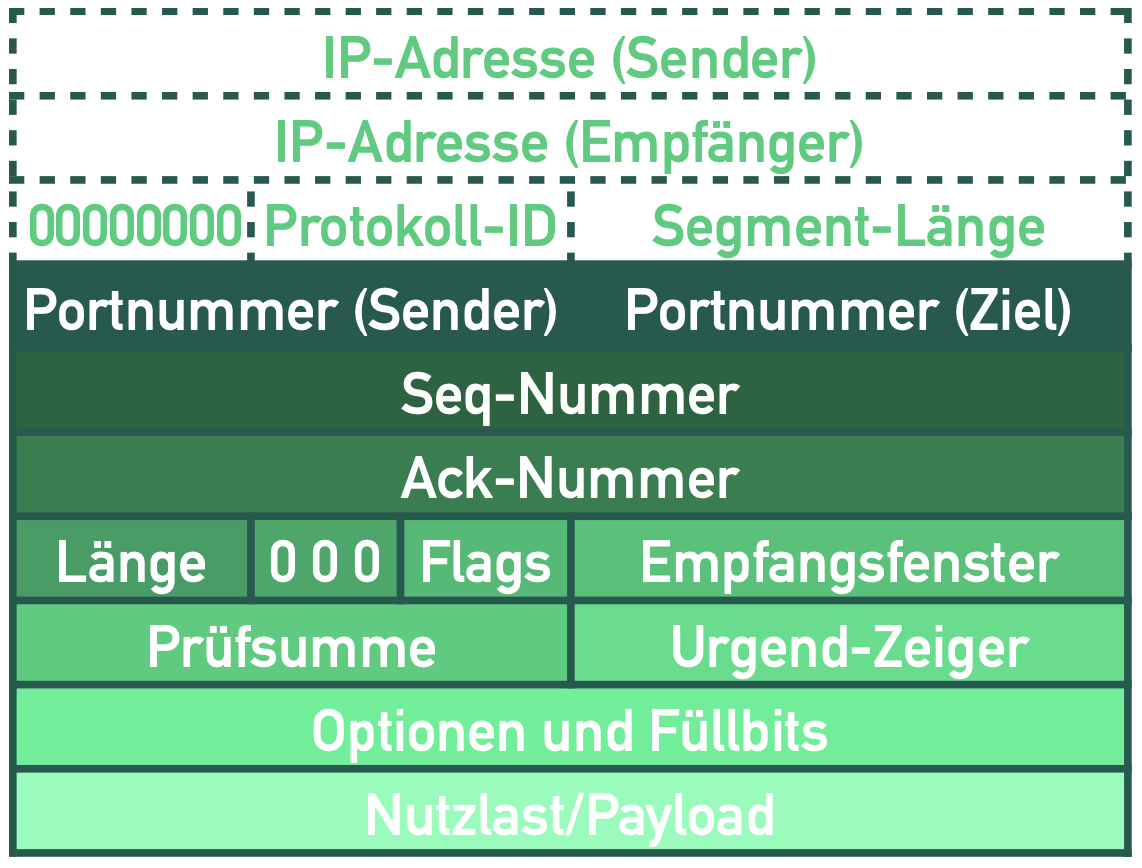
\includegraphics[scale=0.4]{Bilder/TCP.png}
	 \caption{Aufbau des TCP-Pakets. Strichliert der Pseudoheader}
	 \end{figure}
	 \begin{itemize}
	 	\item{Sender Portnummer (16 Bit)}
	 	\begin{itemize}
	 		\item{Portnummer des Senders. 0 falls keine Antwort notwendig ist.}
	 	\end{itemize}
	 	\item{Ziel Portnummer (16 Bit)}
	 	\begin{itemize}
	 		\item{Gibt an, welcher Prozess das Paket enthalten soll.}
	 	\end{itemize}
	 	\item{Sequenznummer (32 Bit)}
	 	\begin{itemize}
	 		\item{Die Sequenznummer des aktuellen Pakets}
	 	\end{itemize}
	 	\item{Acknowledgementnummer (32 Bit)}
	 	\begin{itemize}
	 		\item{Die Nummer, die zurückgeschickt wird, sobald das Paket erhalten wird.}
	 	\end{itemize}
	 	\item{Länge (4 Bit)}
	 	\begin{itemize}
	 		\item{Zusätzlich muss die Länge des Headers übertragen werden, da dieser eine variable Länge haben kann.}
	 	\end{itemize}
	 	\item{Reserviert (3 Bit)}
	 	\begin{itemize}
	 		\item{Für zukünftige Verwendung reserviert.}
	 	\end{itemize}
	 	\item{Flags (9 Bit)}
	 	\begin{itemize}
	 		\item{Es gibt 9 Flags, wobei jedoch nur 3 momentan relevant sind.}
	 		\item{Acknowledgement - Bestätigt Empfang eines Segments.}
	 		\item{Synchronize - Dient zur Synchronisierung der Segmente und zum ersten Verbindungsaufbau.}
	 		\item{Finish - Zeigt, dass keine Daten meh gesendet werden.}
	 	\end{itemize}
	 	\item{Empfangsfenster (16 Bit)}
	 	\begin{itemize}
	 		\item{Anzahl der Bits, welche erhalten werden können.}
	 	\end{itemize}
	 	\item{Prüfsumme (16 Bit)}
	 	\begin{itemize}
	 		\item{Erkennt Übertragungsfehler}
	 	\end{itemize}
	 \end{itemize}
	 \subsubsection{Verbindungsaufbau}
	 TCP baut die Verbindung stets mittels des Three-Way-Handshakes auf. \\
	 Dabei sendet der Sender ein TCP Paket mit der SYN flag gesetzt, um zu zeigen, dass er eine Verbindung aufbauen will. Der Empfänger bestätigt, falls eine Verbindung aufgebaut wird, dass er eine Verbindung aufbauen will und kann, indem er erneut ein TCP Paket mit einem gesetzen SYN aber auch ACK flag. Zur Bestätigung der Bestätigung sendet der Sender erneut ein Bestätigungspaket, weshalb man es auch das Three-Way-Handshake nennt. \\
	 \subsubsection{Datenaustausch}
	 Wenn eine Verbindung aufgebaut ist, können Daten übertragen werden. Dabei ist es essentiell, dass die Sequenz- und Acknowledgementnummer übereinstimmen. Der Sender schickt so immer die Sequenznummer und der Empfänger stets die Acknowledgementnummer. \\
	 Wenn der Sender das erste Segment überträgt, schickt er Sequenznummer 0 mit um zu zeigen, dass dies das erste Segment ist. Wenn der Empfänger dieses Paket erhält, sendet er ein Paket zurück, welches die ACK Flag gesetzt hat und die Sequenznummer plus die Übertragenen Daten als Sequenznummer zurückschickt. \\
	 Also antworter der Empfänger bei einer Sequenznummer von 0 und Daten von 1000 Byte, mit der Acknowledgement 1000 (1000 + 0). \\
	 Der Empfänger wiederum sendet im nächsten Segment die Acknowledgementnummer des letzten Segments als Sequenznummer. \\
	 Dieser Prozess wird wiederholt bis alle Daten übertragen wurden und der Sender die FIN Flag setzt. \\ \\
	 \begin{tabularx}{\textwidth}{| c | c | c | c | c | c | c | X |}
	 	\toprule
	 	Nachricht & ACK & FIN & SYN & Nutzlast & Seq-Nummer & Ack-Nummer & \\ \midrule
	 	 1 & 1 & 0 & 0 & 50 & 0 & 0 & Da hier Daten übertragen werden, ist die SYN Flag nicht mehr gesetzt. \\ \hline
	 	2 & 1 & 0 & 0 & 200 & 0 & 50 & Die Ack-Nummer aus Nachricht 1 wird als Seq-Nummer von Nachricht 2 verwendet und die Nutzlast von Nachricht 1 als Ack-Nummer von Nachricht 2 \\ \hline
	 	3 & 1 & 0 & 0 & 100 & 50 & 200 & Die Ack-Nummer von Nachricht 2 wird als Seq-Nummer von Nachricht 3 verwendet und die Nutzlast von Nachricht 2 als Ack-Nummer von Nachricht 3 \\ \hline
	 	4 & 1 & 1 & 0 & 200 & 200 & - & Die Ack-Nummer aus Nachricht 3 wird wieder als Seq-Nummer von Nachricht 4 übernommen. Es wird keine Ack-Nummer zurückgesendet, da es das letzte Paket ist. \\
	 	\bottomrule
	 \end{tabularx} \\
	 \subsubsection{Verbindungsabbau}
	 Wenn die Verbindung geschlossen werden soll, wird ein TCP Paket mit der FIN Flag gesetzt. Dieses wird wiederum von dem Empfänger bestätigt und erneut vom Sender bestätigt. Somit funktioniert dieser auch nach dem Three-Way-Handshake Prinzip. 
	 \subsubsection{Flusskontrolle (Flow Control)}
	 Flusskontrolle erlaubt die Sendegeschwindigkeit dynamisch einzustellen. Das ist relevant wenn das Netzwerk schneller überträgt als die Verarbeitung geschieht, da der Empfänger sonst für das nächste Segment noch nicht bereit ist und dieses somit verloren geht. Ein Weg um dieses Problem zu lösen, ist das Segment erneut zu senden, falls nötig. \\
	 Strategien hierfür sind unter anderem Stop-And-Wait und das Sliding Window.
	 \paragraphlb{Stop-And-Wait}
	 Der Sender hat einen Timeout, nach welchem er das Segment erneut sendet, falls das Acknowledgement nicht rechtzeitig eintrifft. Dieses System ist zwar sehr simpel, jedoch auch relativ ineffizient und geht nur auf die Bedürfnisse des Senders ein. Deshalb wird dieses Verfahren heute größenteils nicht mehr verwendet.
	 \paragraphlb{Sliding Window}
	 Eine beduetend attraktivere Strategie ist das Sliding Window. Dabei wird die Größe des Empfangsfensters als Referenz verwendet um zu wissen, wie viele Daten noch übertragen werden kann. Dabei erwartet der Sender nur eine Acknowledgement Antwort sobald das Empfangsfenster gefüllt ist, welche dadurch auch in eine Antwort gebündelt werden kann. Nur wenn der Sender nach Füllen des Fensters keine Antwort erhält, wird erneut gesendet, wobei dann alle Segmente des Fensters erneut gesendet werden. \\
	 Da Acknowledgements gebündelt werden, überträgt der Empfänger nur die Acknowledgement wenn alle Segmente darunter auch erhalten wurden. Falls zum Beispiel das dritte Segment verloren geht, antworter der Empfänger stets mit einem Acknowledgement des zweiten Segments, selbst wenn der Sender bereits Segmente 4, 5 und 6 gesendet hat und diese auch empfangen wurden. Wenn der Sender dann nach Ablauf des Fensters das dritte Segment erneut sendet, wird der Empfänger danach das 6. Segment bestätigen, da dieser diese zwischengespeichert hat.
	 \subsubsection{Vor- und Nachteile}
	 Da TCP umfangreiche Sicherheits- und Datensicherungsmaßnahmen setzt, ist die Übertragung auch mit größerer Latenz und größerem Aufwand verbunden. Manchmal ist es jedoch nicht vonnöten sicherzustellen, dass jedes Segment korrekt übertragen wurde, wie zum Beispiel bei Streaming. In solchen Fällen wird dann UDP verwendet. Wenn es jedoch wichtig ist, dass die übertragenen Daten korrekt und komplett übertragen werden, sollte man TCP verwenden. 
	 \section{Anwendungsschicht}
	 Das OSI-Modell definiert zwischen der Transport- und Anwendungsschicht noch die Sitzungsschicht und die Darstellungsschicht, welche jedoch oft ignoriert werden, da die anderen beiden Schichten diese Aufgaben übernehmen können.\\
	 Die Anwendungsschicht übernimmt dabei die Zusammenarbeit verschiedener Programme. In der Anwendungsschicht werden auch die eigentlichen Nachrichten und formattiert, welche übertragen werden.
	 \subsection{Sitzungsschicht}
	 Die Sitzungsschicht wäre für den Aufbau, die Überwachung und das Beenden von Sitzungen verantwortlich. Sitzungen sind Verbindungen zwischen Client und Server und bestehen aus Anfragen und Antworten. Dazu werden Session IDs verwendet. Ports der Transportschicht übernehmen diese Rolle jedoch bereits, wodurch in der Realität nur diese verwendet werden.
	 \subsection{Darstellungsschicht}
	 Die Darstellungsschicht regelt die Formatierung der Nachrichten. So könnte theroetisch der Empfänger darüber informiert werden welche Formatierung vorliegt. Jedoch wird diese Aufgabe wiederum von Anwendungsprotokollen übernommen.
	 \subsection{Domain Name System (DNS)}
	 Wenn man in einem Browser eine Internetadresse eingibt, kann diese nicht direkt von dem Netzwerk verwendet werden sondern muss zuerst in einer IP-Adresse umgewandelt werden. Die URL ist eigentlich nur ein Platzhalter für eine IP-Adresse, welche dynamisch ersetzt wird. \\
	 \subsubsection{hosts}
	 Als das Internet noch eine überschaubare Größe besaß, wurde ein lokales File, welches jeder Computer besaß namens \verb|hosts| verwendet. Dieses enthält heutzutage nur noch die Loopback-Adresse und ein paar weitere lokale Adressen, war jedoch ursprünglich dazu gedacht, alle nötigen Verbindungen darin abzuspeichern. \\
	 Als Ersatz für dieses System wurde das Domain Name System geschaffen. DNS ist ein dezentrales, hierarchisches System zur Auflösung von URLs. Dezentral, weil es keine zentrale Datenbank gibt und die Information auf vielen tausenden Nameservern abgespeichert wird. Hierarchisch, da verschieden Nameserver einander über- oder untergeordnet sind. \\
	 Wenn ein Client auf eine Webadresse zugreifen will, stellt dieser automatisch eine Anfrage an einen DNS um diesen in eine IP-Adresse zu übertragen. Wenn die Domain gefunden werden kann, wird die IP-Adresse retourniert, sonst versucht dieser DNS es von einem übergeordneten Server abzufragen. Wenn die höchste DNS Instanz auch keine Antwort liefern kann, wird ein Fehler zurückgegeben. \\
	 \subsubsection{Namensraum}
	 \begin{figure}[H]
	 \centering
	 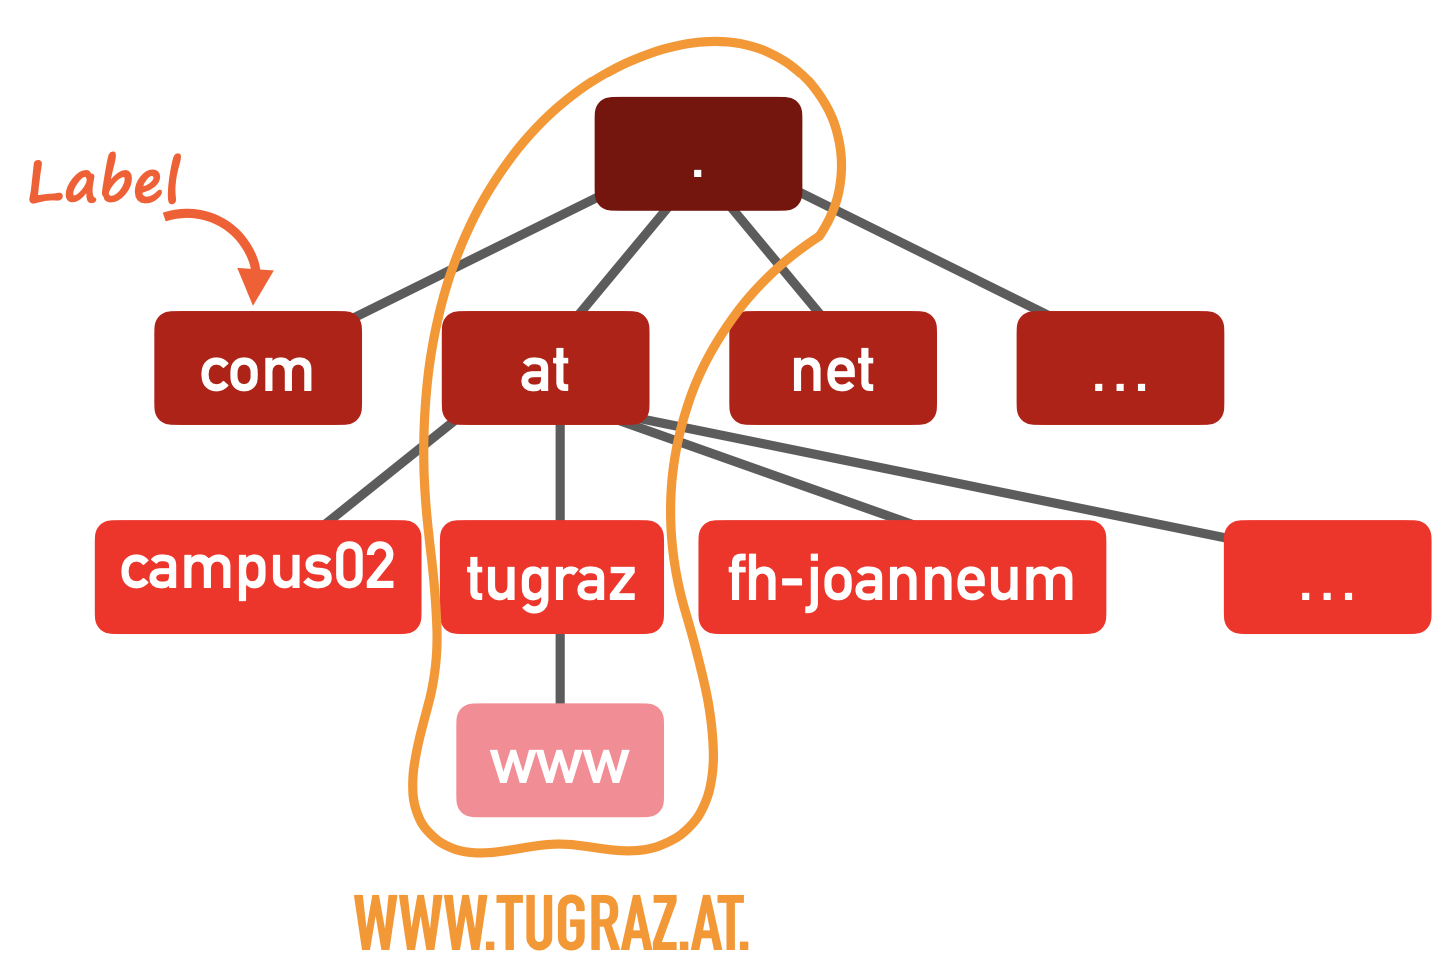
\includegraphics[scale=0.3]{Bilder/URL.png}
	 \caption{Ein URL Baum, welcher zu www.tu-graz.at auflöst.}
	 \end{figure}
	 Die Domain hat einen Namensraum, wodurch sie über verschiedene Levels verfügt. Dabei wird diese in einem Baum aufgebaut und eine URL besteht jeweils aus einem Knoten des Baumes, getrennt durch einen Punkt. Eine URL sollte eigentlich zusätzlich noch einen Punkt am Ende der URL haben, dieser wird jedoch meist weggelassen. \\
	 \begin{figure}[H]
	 \centering
	 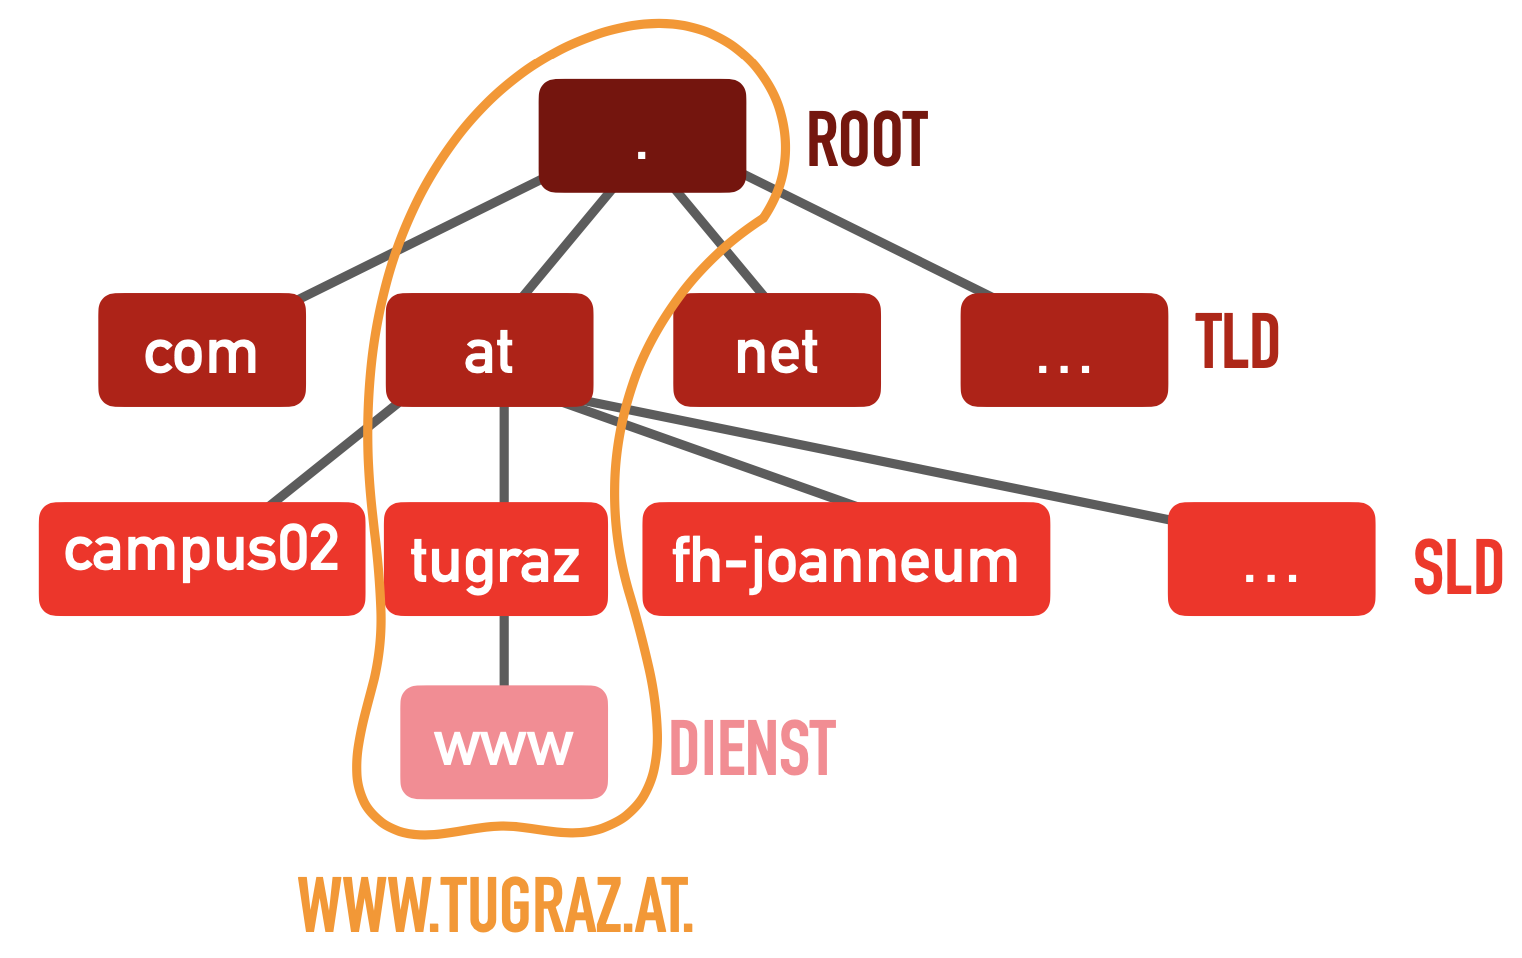
\includegraphics[scale=0.3]{Bilder/DNS.png}
	 \caption{Hierarchien einer URL}
	 \end{figure}
	 Alle URLS führen in der root zusammen, welche aus einem Punkt besteht. Aus diesem Grund sollte am Ende jeder URL ein Punkt stehen, welcher jedoch optional ist. \\
	 Ausgenommen des roots besteht eine URL stets aus einer Top-Level-Domain (TLD), welche das weiteste Netzwerk darstellt. Diese sind meistens Ländercodes wie \verb|.at| oder \verb|.de| aber es gibt viele andere TLDs wie \verb|.org| für Organisationen oder \verb|.com| für Unternehmen. \\
	 Danach kommen Second-Level-Domains (SLD), welche die einzelnen Adressen darstellt und individuell gewählt werden kann. Diese können wiederum in Unterkategorien geteilt werden, was jedoch innerhalb des Servers individuell gehandhabt wird. \\
	 Zuletzte wird der Dienst angegeben über welchen es versendet wird. Das ist meistens World Wide Web (WWW), man kann jedoch über einen Browser zum Beispiel auch SMTP Anfragen verschicken. \\
	 \subsubsection{DNS Server}
	 DNS Server werden in zwei Kategorien geteilt: Autoritative und Nicht-Autoritative Server. \\
	 \paragraphlb{Autoritativ}
	 Autoritative Server sind verantwortlich für eine grobe Zone, wobei es in jeder dieser Zonen mindestens einen gibt. Dabei speichert der Server Zuweisungsinformation in einer Zonendatei um Anfragen zuzweisen zu können. Da ein solcher Server eine sehr große Anfragenlast bearbeiten muss, sind Autoritative DNS Server fast immer in einem Cluster konfiguriert, wodurch die Last auf mehrere Server verteilt werden kann. Das hilft auch dabei die Verzögerung bei Anfragen zu minimieren. \\
	 Die Information für TLDs wird von 13 Name Servern verwaltet, welche von A bis M benannt sind.
	 \paragraphlb{Nicht-Autoritativ}
	 Im Gegensatz dazu stehen Nicht Autoritative Name Server. Diese beziehen ihre Informationen wiederum von anderen DNS Servern, wodurch die Korrektheit der Daten nicht gänzlich gesichert werden kann. \\
	 Solche Server haben zwei Strategien um Informationen von anderen Servern einzuholen:
	 \begin{itemize}
	 	\item{Rekursive Auflösung}
	 	\begin{itemize}
	 		\item{Der Server befragt einen anderen Server, welcher ihn wiederum beauftragt bei einem anderen Server nachzufragen usw.}
	 	\end{itemize}
	 	\item{Iterative Auflösung}
	 	\begin{itemize}
	 		\item{Der Server befragt einen anderen Server, welcher ihm danach mitteilt wo er als nächstes nachfragen sollte, bis er zu seinem Ziel kommt.}
	 	\end{itemize}
	 \end{itemize}
	 Somit sind die grundlegenden Aufgaben eines DNS:
	 \begin{itemize}
	 	\item{Delegieren}
	 	\begin{itemize}
	 		\item{}
	 	\end{itemize}
	 	\item{Caching}
	 	\item{Forwarding}
	 \end{itemize}

	 \subsubsection{Ablauf}
	 Der Ablauf einer Anfrage verläuft nach einer festen Struktur:
	 \begin{enumerate}
	 	\item{Eine Anfrage wird im Browser gesendet.}
	 	\item{Der Browser sieht nach, ob die Adresse lokal verfügbar ist.}
	 	\begin{itemize}
	 		\item{Dabei wird zuerst in dem cache des Browsers nachgesehen (Falls diese bereits vor kurzem aufgerufen wurde.)}
	 		\item{Danach wird in der \verb|hosts| Datei und dem cache des lokalen DNS resolvers nachgesehen. }
	 	\end{itemize}
	 	\item{Falls lokal nichts gefunden wird, fragt er bei dem Default Gateway (Dem Router) nach, da dieser auch einen DNS cache hat.}
	 	\item{Falls der Router keine Antwort hat, wird am Nameserver des ISPs nachgesehen.}
	 	\item{Falls der ISP Nameserver auch keine Antwort hat, wird iterativ an einem root Nameserver nachgesehen.}
	 	\begin{itemize}
	 		\item{Der root nameserver hat eine Zonendatei, wodurch er ungefähr weiß wo sich jede Top-Level-Domain befindet und kann dadurch in etwa zurückgeben wen der Nameserver als nächstes Fragen sollte.}
	 	\end{itemize}
	 	\item{Der ISP Nameserver folgt dieser IP-Adresse und fragt solange weiter bis er zu einem Ergebnis kommt oder der Server sagt, dass diese Adresse nicht existiert.}
	 \end{enumerate}
	 Ein Programm zur Visualisierung der DNS Abfrage ist DIG. Das Programm gibt stets die Liste der möglichen Server zu Abfrage an, sowie welcher Server geantwortet hat. Dabei wird die Liste möglicher Server zur Anfrage angegeben und dann, welcher Server geantwortet hat, wonach die Liste wieder ausgegeben wird. \\
	 \paragraphlb{Umlaute}
	 Da DNS nur mit ASCII Zeichen arbeitet müssen bei anderen Zeichen diese substitutioniert werden. Dabei wird es durch Punycode ersetzt, welcher versucht nicht-ASCII Zeichen darzustellen. Dieser Prozess funktioniert jedoch nicht einwandfrei und wird auch nicht von jedem System unterstützt weshalb es öfter vorkommt, dass eine Adresse mit nicht-ASCII Zeichen auf eine alternative Adresse verweist und diese aufgerufen wird. \\
	 \subsection{Dynamic Host Configuration Protocol (DHCP)}
	 Da jedes Gerät innerhalb eines lokalen Netzwerks eine eigene IP-Adresse braucht, diese sich jedoch ändern können, ist es nötig diese dynamisch zu vergeben. Ein Weg um diese automatisch zu verteilen ist DHCP. Dabei verteilt ein DHCP Server einen Pool an spezifischen IP-Adressen abhängig der verbundenen Geräte. Heutzutage hat jeder Router in der Regel einen eingebauten DHCP Server und vollführt diese Aufgabe automatisch. In größeren Netzwerken wird diese Aufgabe oft von einem dezidierten Server übernommen. \\
	 Da DHCP Broadcasts zur Zuweisung verwendet, müssen der Server und der Client im gleichen Netz liegen. Sollte er in einem anderen Netz liegen, kann ein DHCP Relay verwendet werden um sich zum Server zu verbinden. \\
	 \subsubsection{Funktionsweise}
	 DHCP agiert in vier Schritten: DORA: Discover, Offer, Request, Acknowledge.
	 \begin{enumerate}
	 	\item{Discover}
	 	\begin{itemize}
	 		\item{Ein Client ohne eine IP-Adresse sendet einen Broadcast an das Netzwerk um eine IP-Adresse zu erhalten.}
	 		\item{Dabei wird die Sender IP-Adresse auf 0.0.0.0 gesetzt, da der Client ja momentan noch keine Adresse hat.}
	 	\end{itemize}
	 	\item{Offer}
	 	\begin{itemize}
	 		\item{Jeder erreichbare DHCP Server antworter auf die Anfrage und sendet einen weiteren Broadcast in das Netzwerk um eine IP-Adresse anzubieten. Er sendet erneut einen Broadcast, da der Client ja immer noch keine Adresse besitzt.}
	 	\end{itemize}
	 	\item{Request}
	 	\begin{itemize}
	 		\item{Der Client nimmt ein Angebot an und sendet erneut als Broadcast die Annahme seiner neuen Adresse.}
	 		\item{Es wird als Broadcast versendet, da es sein könnte, dass mehrere DHCP-Server gleichzeitig eine Anfrage verschickt haben und diese darüber informiert werden, dass ihr Angebot nicht angenommen wurde.}
	 	\end{itemize}
	 	\item{Acknowledge}
	 	\begin{itemize}
	 		\item{Der DHCP Server sendet wiederum als Broadcast die Anfrage und bestätigt diese indem sie in den Adresspool eingefügt wird.}
	 		\item{Falls alle Adressen vergeben sind, kann keine Adresse vergeben werden.}
	 	\end{itemize}
	 \end{enumerate}
	 \subsubsection{Lease Time}
	 Jede per DHCP erteilte IP-Adresse besitzt ein Verfallsdatum. (Lease Time) Der Server teil dem Client dabei das Ablaufdatum mit und es ist dessen Aufgabe diese in Intervallen zu erneuern. Das stellt sicher, dass nur aktive Hosts weiter abgespeichert werden.
	 \subsection{Hypertext Transfer Protocol (HTTP)}
	 HTTP ist, gemeinsam mit der URL (Uniform Resource Locator) und HTML (Hypertext Markup Language), die Grundlage für das World Wide Web (WWW). HTTP wird größtenteils dafür verwendet um eine Webseite von einem Webserver in einen Browser zu laden. Dabei ist HTTP zustandslos, wodurch keine Information aus früheren Anfragen benötigt wird und jegliche Information mit jeder Anfrage übertragen wird.
	 \subsubsection{Verbindungsaufbau}
	 Bei dem Aufbau einer Verbindung wird die URL ausgesendet und von dem DNS in eine IP-Adresse umgewandelt. Danach öffnet der Browser als Client eine \verb|http| Verbindung zu dem relevanten Webserver und vollführt den aus TCP bekannten Three-Way-Handshake. Danach wird ein HTTP-Request übertragen, welche verschiedene Befehle wie \verb|get|, \verb|post| oder andere enthalten kann. Wenn man eine Website aufruft wird dabei ein \verb|get| request gepostet. Sobald die Verbindung aufgebaut wird, überträgt der Server die angefragte Datei und gibt den Statuscode 200 (OK) zurück. In der Theorie wird danach, gleich wie bei TCP die Verbindung wieder geschlossen. Jedoch ist es heute durchaus verbreitet, dass HTTP Verbindungen persistent sind, also eine gewisse Zeit aufrechterhalten werden.
	 \subsection{E-Mail}
	 Die Übertragung von E-Mails hat mehrere Komponenten: \\
	 Man braucht natürlich einen E-Mail Client, welcher empfangene E-Mails für später aufbewahrt. Jedoch benötigt man auch einen Mail Server, welcher den Client über neue E-Mails in Kenntnis setzt. \\
	 Diese zwei Komponenten benötigen Protokolle um ihre Daten zu übertragen:
	 \begin{itemize}
	 	\item{Übertragung zwischen Mail Servern}
		\begin{itemize}
	 		\item{Simple Mail Transfer Protocol - SMTP}
		 	\begin{itemize}
		 		\item{Wird verwendet um Mails zwischen Servern auszutauschen. Dabei kann es einen anderen Eingangs- als Ausgangsserver geben.}
		 	\end{itemize}
		\end{itemize}
		\item{Übertragung zwischen Mail Server und Mail Client}
		\begin{itemize}
			\item{Post Office Protocol (POP)}
			\begin{itemize}
				\item{Kann am Mail Server auflisten, abholen und löschen}
			\end{itemize}
			\item{Internet Message Access Protocol (IMAP)}
			\begin{itemize}
				\item{Kann zusätzlich zur POP Funktionalität auch eine Ordnerstruktur definieren und sich zwischen verschiedenen Geräten (Wie z.B. Laptop und Handy) synchronisieren.}
			\end{itemize}
			\item{Im Falle eines Onlinepostfachs (Wie GMail) wird auch HTTP zur Übertragung verwendet.}
		\end{itemize}
	 \end{itemize}
	 \subsubsection{Ablauf}
	 Wenn eine E-Mail von einem Client gesendet wird, wird diese per SMTP an den Mail Server übertragen. Dieser überträgt die Nachricht wieder per SMTP an den Ziel Mail Server, baut jedoch zuerst eine TCP Übertragung auf, wonach er die Nachricht überträgt. Der Mail Server speichert die Mail und wartet, bis der Empfänger das nächste Mal seine Mails abruft. Sobald dies der Fall ist, wird die Nachricht per POP oder IMAP an den Mail Client übertragen.
	 \section{IPv6}
	 NAT ist nur vonnöten, da IPv4 nur 4,3 Milliarden IP-Adressen definieren kann. Als Nachfolger wurde bereits vor einiger Zeit IPv6 standardisiert, welche zusätzlich zu besseren Sicherheitsmaßnahmen auch einen bedeutend größeren Adressbereich definiert. So hat IPv4 eine 32-Bit Adresse, IPv6 jedoch 128-Bit was zu einem Adressbereich von $3,4*10^38$ führt und für die nahe Zukunft genug Adressen bieten könnte. \\
	 Da IPv6 aus 128-Bit besteht, ist dessen Darstellung in Binär etwas unhandlich. Aus diesem Grund werden IPv6 Adressen in Hexadezimal dargestellt, wobei 8 Blöcke mit je 16 Bit pro Block geschrieben werden. Die resultierender Hexadezimalzahl ist trotzdem noch relativ lang: \verb|2001:0DB8:0000:0000:0008:0800:200C:417A|.\\
	 Aus diesem Grund gibt es Vereinfachungsregeln:
	 \begin{itemize}
	  	\item{Führende Nullen innerhalb eines Blockes können weggelassen werden: \verb|2001:DB8:0:0:8:800:200C:417A|}
	  	\item{Wenn ein Block nur aus Nullen besteht, kann dieser komplett weggelassen werden: \verb|2001:DB8::8:800:200C:417A|}
	  \end{itemize} 
	  IPv6 Adressen bestehen aus 2 Teilen: Dem Präfix und dem Interface Identifier (II), wobei diese jeweils die ersten und letzten 64 Bit sind. Der Präfix wird vom ISP vergeben und gibt das Netz an. Der Interface Identifier kennzeichnet dabei die Teilnehmer innerhalb eines Netzes. Dieser kann manuell festgelegt oder von DHCP vergeben werden. \\
	  Der II kann durch einen / am Ende der Adresse angegeben werden
	  \subsection{Spezielle Adressen}
	  \cprotect\subsubsection{Link Local Unicast Adresse - \texorpdfstring{\verbĦFE80::/10Ħ}{      } }
	  Sind nur innerhalb eines lokalen Netzes gültig und müssen neben globalen IPv6 Adressen angegeben werden. Diese Adresse kann verwendet werden um MAC Adressen anderer Geräte innerhalb des lokalen Netzes erfragt werden. (Ähnelt ARP)
	  \cprotect\subsubsection{Loopback - \verb|::1/128| }
	  Die Adresse des eigenen Standorts
	  \cprotect\subsubsection{Multicast Adressen - \texorpdfstring{\verbĦFF01::1/FF02::1Ħ}{} }
	  Da es keine Broadcast Adresse gibt, muss dies durch Multicast Adressen realisiert werden. 
	  \subsection{IPv6 Header}
	  Der IPv6 Header besteht aus zwei Teilen: Dem Header mit einer fixen Größe sowie dem Extension Header, welcher eine variable Größe haben kann und in Summe nur in das Paket passen muss. 
	  \begin{figure}[H]
	  \centering
	  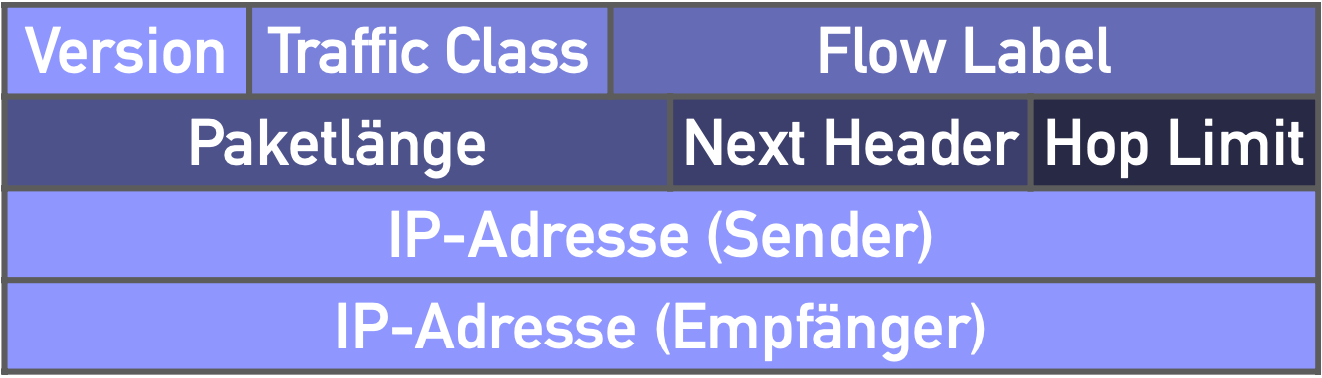
\includegraphics[scale=0.4]{Bilder/IPv6.png}
	  \caption{Der Hauptheader eines IPv6 Pakets}
	  \end{figure}
	  Der Hauptheader hat eine konstante Größe von 40 Byte und inkludiert folgende Komponenten:
	  \begin{itemize}
	  	\item{Die Protokollversion (4 Bit)}
	  	\begin{itemize}
	  		\item{Version 6 für IPv6}
	  	\end{itemize}
	  	\item{Die Traffic Class (8 Bit)}
	  	\begin{itemize}
	  		\item{Gibt die Priorität des Pakets an}
	  	\end{itemize}
	  	\item{Das Flow Label (20 Bit)}
	  	\begin{itemize}
	  		\item{}
	  	\end{itemize}
	  \end{itemize}

	  \subsection{Kompatibilität IPv4 vs IPv6}
	  IPv4 ist in einigen Teilen kompatibel zu IPv6, jedoch nicht in allen. So kann man in beiden TCP, UDP und DNS verwenden, jedoch nicht ICMP und DHCP, wofür es eigene Protokolle gibt (ICMPv6 und DHCPv6). Zusätzlich hat IPv6 kürzere Header, wodurch es effizienter übertragen werden kann. Auch hat IPv6 einen grundlegenden Sicherheitsgedanken, wodurch dieser von Anfang an inkludiert wurde, während es bei IPv4 erst im Nachhinein hinzugefügt wurde. IP-Adressen würden zwar weiterhin relativ ineffizient verteilt werden. \\
	  \subsubsection{Interoperabilität}
	  IPv4 und IPv6 sind zwar inkompatibel zueinander, können jedoch nebeneinander existieren. Wenn man ein IPv6 Gerät in einem IPv4 Netz verwenden will gibt es jedoch zwei Wege um dies zu ermöglichen. Diese Verfahren nennen sich Dual Stacking und Tunneling.
	  \begin{itemize}
	  	 	\item{Dual Stack}
	  	 	\begin{itemize}
	  	 		\item{Jeder Router hat sowohl eine IPv4, als auch eine IPv6 Adresse. Wenn eine IPv6 Adresse auf einen IPv4 Server zugreifen will, ersetzt der Router die Adresse durch die eigene um eine Kommunikation zu ermöglichen.}
	  	 	\end{itemize}
	  	 	\item{Tunneling}
	  	 	\begin{itemize}
	  	 		\item{Wenn ein IPv6 Paket zu einem anderen IPv6 Server gesendet wird, das Netz dazwischen jedoch nur IPv4 unterstützt, kann man das Paket in ein IPv4 Paket verpacken und so über das IPv4 Netz verschicken.}
	  	 	\end{itemize}
	  \end{itemize}	
	  \section{Netzwerksicherheit} 
	  Da man im Internet mit theoretisch allen anderen Benutzern verbunden ist, muss man auf die Sicherheit seiner Daten achten. Da das Internet eine dezentrale Struktur hat, ist es schwer eine umfassende Kontrolle durchzuführen. Jedes Jahr werden millionen an Daten gestohlen, oft über öffentliche Netzwerke.
	  \subsection{Pfeiler der Netzwerksicherheit}
	  \subsubsection{Authentizität}
	  Sicherstellen, dass der Kommunikationspartner tatsächlich der ist, für den er sich ausgibt. Gleich wie man sich oft mit einem Führerschein oder Pass ausweisen muss, kann das auch im Internet geschehen. Dadurch kann man auch kontrollieren, wer welche Berechtigungen hat.
	  \subsubsection{Vertraulichkeit}
	  Kein dritter sollte die Kommunikation einsehen können. (Mittels Verschlüsselung)
	  \subsubsection{Integrität}
	  Prüfen und Sicherstellen, dass Daten nicht manipuliert sind.
	  \subsubsection{Verfügbarkeit}
	  Vertrauen, dass der Kommunikationspartner verfügbar ist, wenn nötig.
	  \subsection{Verschlüsselungsverfahren}
	  Bei der Verschlüsselung gibt es zwei Verfahren: Symmetrische und Asymmetrische Verschlüsselungsverfahren.
	  \subsubsection{Symmetrische Verschlüsselung}
	  Bei der symmetrischen Verschlüssel wird der selbe Schlüssel verwendet um die Nachricht sowohl zu ver- als auch zu entschlüsseln. Solche Verfahren werden schon seit tausenden Jahren verwendet, wie der Caesar Cypher, welcher anscheinend schon bei den Römern Verwendung fand. Solche Verschlüsselungsverfahren sind heutzutage sehr unsicher und sollten nicht mehr verwendet werden.
	  \subsubsection{Asymmetrische Verschlüsselung}
	  Im Gegensatz dazu gibt es asymmetrische Verschlüsselungsverfahren. Dabei gibt es jeweils zwei Schlüssel: Einen zum ver- und einen zum entschlüsseln. Einer davon ist der \textbf{private} und einer der \textbf{public} key. Der public key ist öffentlich zugänglich und kann im Internet übertragen werden. Der private key hingegen darf \textit{nie} an die Öffentlichkeit gelangen. So kann sichergestellt werden, dass nur der Empfänger die Nachricht lesen kann. Dabei verschlüsselt der Sender die Nachricht mit dem public key wonach diese nur mit dem private key des Empfängers wieder entschlüsselt werden kann. \\
	  \subsection{Zertifikate}
	  Mit Zertifikaten kann man sicherstellen, dass ein Benutzer auch wirklich der ist, für den er sich ausgibt. Solche Zertifikate werden von Certification Authorities (CA) ausgegeben. Eine solche CA ist zum Beispiel A-Trust. Diese speichern ein Zertifikat auf dem PC, welches von anderen dann überprüft werden kann.
	  \subsection{Übertragungsprotokolle}
	  Sichere Übertragungsprotokolle sind ein Weg gegenseitige Authentifizierung und Verschlüsselung sicherzustellen. Es gibt jedoch stets ein Risiko, welche meist von dem Benutzer selbst ausgeht. Firmenfremde Geräte können auch die Sicherheit des Systems beeinträchtigen.
	  \subsection{Angriffsszenarien}
	  \subsubsection{Denial of Service Attack (DOS)}
	  Ein Denial of Service Attack (DOS) zielt darauf an den Server zu überlasten indem in kurzer Zeit sehr viele Anfragen gestellt werden. Das hat das Ziel den Server offline zu zwingen oder durch die Überlastung eine Sicherheitslücke auszunutzen. Da Anfragen von einem Server jedoch einfach verhindert werden können, gibt es auch den Distributed Denial of Service (DDOS) Attack, bei welchem viele verschiedene Clients von vielen verschiedenen IP-Adressen gleichzeitig Anfragen versenden, wodurch der Server nicht weiß, welche Anfragen echt sind und welche nicht.
	  \subsubsection{Man in the Mittle (MITM)}
	  Bei dem Man in the Middle klinkt sich ein Angreifer zwischen die Übertragung zweier Parteien und greift jegliche Kommunikation ab. Der Angreifer hat dabei komplette Kontrolle über den Datenverkehr. Da jedoch bald ersichtlich werden würde, dass etwas nicht stimmt, wenn die Anfragen nicht ankommen, liest der Angreifer diese oft nur aus und gibt sie dann weiter. In einem anderen Seznario können Daten jedoch auch 
	  \subsection{Layer Attacks}
	  Es gibt spezifische Angriffsmöglichkeiten für die einzelnen Schichten des OSI Modells.
	  \subsubsection{Mac Flooding - Sicherungsschicht (DOS)}
	  Ein Switch versucht stets bekannte MAC Adressen zu speichern. Dieses Verhalten kann man ausnützen um die MAC Tabellen zu überfüllen, da diese natürlich auch nur einen begrenzten Speicher hat. Wenn die Tabelle voll ist, haben Switches normalerweise zwei Wege um weiterzuarbeiten: Entweder alle Frames werden verworfen oder alle Pakete werden gebroadcastet, da der Switch nicht mehr weis, wo diese hin müssen. Um dies zu verhindern können Server MAC Adressen zertifizieren und alle anderen werden nicht angenommen.
	  \subsubsection{ARP Spoofing - Sicherungsschicht (MITM)}
	  Mit dem ARP Protokoll kann man mittels Broadcast die MAC Adressen von Benutzern im lokalen Netzwwerk herausfinden. Ein Angreifer kann auf einen solchen ARP Broadcast antworten, obwohl er nicht die richtige IP Adresse hat, und somit als Ziel für Pakete gespeichert werden. Dadurch erhält er die Daten die eigentlich an einen anderen Benutzer gehen sollten. \\
	  Nachdem das Paket abgefangen wurde, kann man dann die Nachricht entweder nur auslesen oder manipulieren. Danach wird mittels MAC Spoofing die MAC Adresse des Pakets geändert und an den wahren Empfänger versendet. Dadurch weiß der Empfänger nicht, dass die Nachricht abgefangen wurde.
	  \subsubsection{IP Fragmentierung - Vermittlungsschicht (DOS)}
	  Da ein IP Paket in viele kleine Pakete aufgespalten werden kann, und der Empfänger diese speichert bis er das ganze Paket erhalten hat, kann man stets unvollständige IP Pakete verschicken um so den Speicher des Opfers zu überlasten.
	  \subsubsection{IP Spoofing - Vermittlungsschicht (MITM + DOS)}
	  IP hat grundsätzlich keine Verschlüsselung, wodurch die Sender und Empfänger IP Adresse einsehbar ist. So kann man die Sender IP Adresse zur eigenen IP Adresse ändern um so die Antwort zu erhalten. Das kann man einerseits verwenden um Daten abzufangen und auszulesen, aber auch um effektivere DOS Angriffe durchzuführen, da das Opfer nie wissen kann, welches Paket vom Angreifer kommt und welches nicht. Ein Weg dies zu umgehen ist eine Firewall im Router, welche jegliche Anfragen von außen an PCs im System verwirft.
	  \subsubsection{SYN Flood - Transportschicht (DOS)}
	  Bei einem TCP Three-Way Handshake wird mit einer SYN Anfrage eine Verbindungsanfrage gestellt. Man kann jedoch wiederholt SYN Anfragen schicken, ohne auf die ACK Antwort zu antworten. Da ein Server speichert, von wem eine TCP Anfrage eingegangen ist, kann dies den Speicher des Opfers schnell füllen und eventuell sogar Server zum Absturz bringen. Eine Gegenmaßnahme sind intelligente Firewalls, welche das Netzwerk analysieren und solche Floods unterdrücken.
	  \subsubsection{DNS Spoofing und Cache Poisoning - Anwendungsschicht (MITM)}
	  Ein DNS Server ist dafür verantwortlich eine IP Adresse für eine URL zurückzugeben. Da DNS Anfragen jedoch nicht verschlüsselt sind und bei einer DNS Anfrage nicht überprüft wird, ob der Server den man fragt, auch die Antwort sendet, kann man die Anfrage manipulieren und so einen anderen Server als Ziel angeben. Dieser kann die erwartete Website dann so genau wie möglich imitieren und so zum Beispiel eine Phishing Attacke durchzuführen.
	  \subsubsection{DHCP Spoofing - Anwendungsschicht (DOS + MITM)}
	  DHCP Server vergeben IP Adressen an Teilnehmer im lokalen Netzwerk. Ein Angreifer kann sich jedoch als DHCP Server ausgeben und dem Client eine falsche IP Adresse ausgeben. Dabei ist der PC des Angreifers das Default Gateway. Im Falle eines DOS werden Anfragen danach einfach nicht weitergegeben, wodurch dieser mit niemandem mehr kommunizieren kann. Bei einem MITM kann der Angreifer Anfragen an das Default Gateway auslesen und dann an das echte Ziel weiterleiten.
	  \subsubsection{DHCP Starvation - Anwendungsschicht (DOS)}
	  Da ein Subnetz stets nur eine begrenzte Menge an Hosts gleichzeitig haben kann, kann man die DHCP Tabelle des DHCP Servers so anfüllen, dass keine neuen Clients aufgenommen werden können.
	  \subsection{Transport Layer Security (TLS)}
	  TLS ist der Nachfolger des Secure Socket Layers (SSL) und dient der Authentifizierung und Verschlüsselung von Internetverbindungen. TLS wird dabei im TCP/IP Modell dem Transport Layer zugeschrieben, während es im OSI Modell der Sitzungsschicht zugeordnet wird. Die Authentizität eines Benutzers wird dabei mit den vorhin erwähnten Zertifikaten sichergestellt. TLS kann auf verschiedene unsichere Protkolle angewandt werden, um diese zu verschlüsseln. So kann mittels TLS HTTP zu HTTPS werden, welche eine verschlüsselte Verbindung zu Websites aufbaut.
	  \subsubsection{Handshake}
	  TLS beginnt seine Verbindung mittels eines Handshakes. 
	  \begin{itemize}
	  	\item{Client Hello}
	  	\begin{itemize}
	  		\item{Bei der ersten Verbindung baut der Client die Verbindung zum Server auf.}
	  		\item{Enthält das Zertifikat des Clients, die TLS Version sowie die Cypher Suit (Das Verschlüsselungsverfahren) und eine Menge an zufälligen Zahlen (Client Random)}
	  	\end{itemize}
	  	\item{Server Hello}
	  	\begin{itemize}
	  		\item{Der Server überprüft das Zertifikat mit einer CA und sendet daraufhin sein eigenes Zertifikat sowie das Verschlüsselungsverfahren und wieder eine Menge an zufälligen Zahlen (Server Random)}
	  	\end{itemize}
	  	\item{Premaster Secret}
	  	\begin{itemize}
	  		\item{Wenn beide Zertifikate gültig sind, erstellt der Client eine weitere zufällige Bitfolge (Premaster Secret) und verschlüsselt diese mit dem Public Key des Servers.}
	  		\item{Der Server entschlüsselt das Premaster Secret.}
	  		\item{Sowohl der Server als der Client erstellen mittels Client Random, Server Random und Premaster Secret einen Sessionschlüssel, welcher ab nun verwendet wird um sich gegenseitig zu verifizieren.}
	  	\end{itemize}
	  	\item{Server Done}
	  	\begin{itemize}
	  		\item{Der Server ist bereit zur Kommunikation}
	  	\end{itemize}
	  	\item{Client Done}
	  	\begin{itemize}
	  		\item{Der Client ist bereit zur Kommunikation}
	  	\end{itemize}
	  \end{itemize}
	  \subsection{Firewalls}
	  Firewalls sind eine weitere Sicherheitsmaßname um schädliche Pakete abzuhalten. Diese blockieren Pakete anhand von Regeln. Diese Regeln lassen normalerweise Anfragen von innen nach außen zu, jedoch nicht umgekehrt. Dabei müssen diese jedoch wissen, welche Pakete von außen als Antwort auf eine Anfrage von innen kommen und diese zulassen. Viele Firewalls haben deshalb eine Statusliste zur Überprüfung der Kommunikation.












\end{document}